
%!TEX root = ../thesis.tex
%*******************************************************************************
%****************************** Second Chapter *********************************
%*******************************************************************************

\newcommand{\ba}{\mathbf{a}}
\newcommand{\bb}{\mathbf{b}}
\newcommand{\bd}{\mathbf{d}}
\newcommand{\bw}{\mathbf{w}}
\newcommand{\bx}{\mathbf{x}}
\newcommand{\by}{\mathbf{y}}
\newcommand{\Exp}[2]{\mathbb{E}_{#1}\left[#2\right]}
\newcommand{\Var}[2]{\text{Var}_{#1}\left[#2\right]}
\newcommand{\Cov}[2]{\text{Cov}_{#1}\left[#2\right]}
\newcommand{\Corr}[2]{\text{Corr}_{#1}\left[#2\right]}

\newcommand{\bA}{\mathbf{A}}
\newcommand{\bB}{\mathbf{B}}
\newcommand{\bV}{\mathbf{V}}
\newcommand{\bW}{\mathbf{W}}
\newcommand{\bv}{\mathbf{v}}

\newcommand{\bphi}{\mathbf{\phi}}
\newcommand{\bt}{\mathbf{\theta}}
\newcommand{\bdelta}{\mathbf{\delta}}
\newcommand{\beps}{\mathbf{\epsilon}}
\newcommand{\q}{q_\mathbf{\phi}}
\newcommand{\bmu}{\mathbf{\mu}}
\newcommand{\bsigma}{\mathbf{\sigma}}
\newcommand{\bSigma}{\mathbf{\Sigma}}

\newcommand{\D}{\mathcal{D}}

\newcommand{\eqnr}{\addtocounter{equation}{1}\tag{\theequation}}

\chapter{Background}

\ifpdf
    \graphicspath{{Chapter2/Figs/Raster/}{Chapter2/Figs/PDF/}{Chapter2/Figs/}}
\else
    \graphicspath{{Chapter2/Figs/Vector/}{Chapter2/Figs/}}
\fi


\fbox{
    \parbox{\textwidth}
    {
       Chapter Overview
        \begin{itemize}
            \item Neural Networks and Convolutional Neural Networks.
            \item Concepts overview of Variational Inference, and local reparameterization trick in Bayesian Neural Network.
            \item Backpropagation in Bayesian Networks using Bayes by Backprop.
            \item Estimation of Uncertainties in a network.
            \item Pruning a network to reduce the number of overall parameters without affecting its performance.
        \end{itemize}
    }
}

\pagebreak

\section{Neural Networks}
\subsection{Brain Analogies}

A perceptron is conceived as a mathematical model of how the neurons function in our brain by a famous psychologist Rosenblatt. According to Rosenblatt, a neuron  takes a set of binary inputs (nearby neurons), multiplies each input by a continuous-valued weight (the synapse strength to each nearby neuron), and thresholds the sum of these weighted inputs to output a 1 if the sum is big enough and otherwise a 0 (the same way neurons either fire or do not fire).

\begin{figure}[H]
\begin{center}
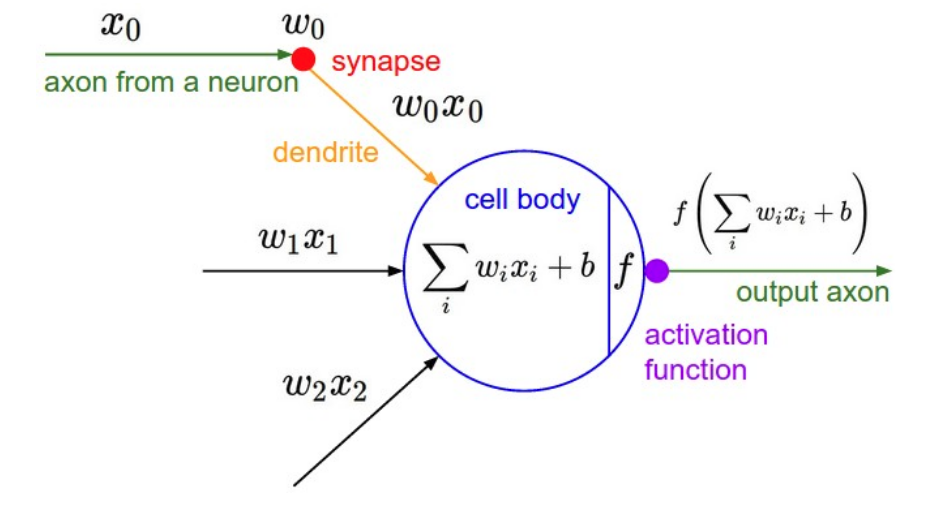
\includegraphics[height=.28\textheight]{Chapter2/Figs/NeuralNetwork.png}
\label{fig:Neural_Network}
\caption{Biologically inspired Neural Network \cite{karparthy}}
\end{center}
\end{figure}

\subsection{Neural Network}

Inspired by the biological nervous system, the structure of an Artificial Neural Network (ANN) was developed to process information similar to how brain process information. A large number of highly interconnected processing elements (neurons) working together makes a Neural Network solve complex problems. Just like humans learn by example, so does a Neural Network. Learning in biological systems involves adjustments to the synaptic connections which is similar to weight updates in a Neural Network. 

A Neural Network consists of three layers: input layer to feed the data to the model to learn representation, hidden layer that learns the representation and the output layer that outputs the results or predictions. Neural Networks can be thought of an end to end system that finds patterns in data which are too complex to be recognized by a human to teach to a machine. 


\begin{figure}[H]
\begin{center}
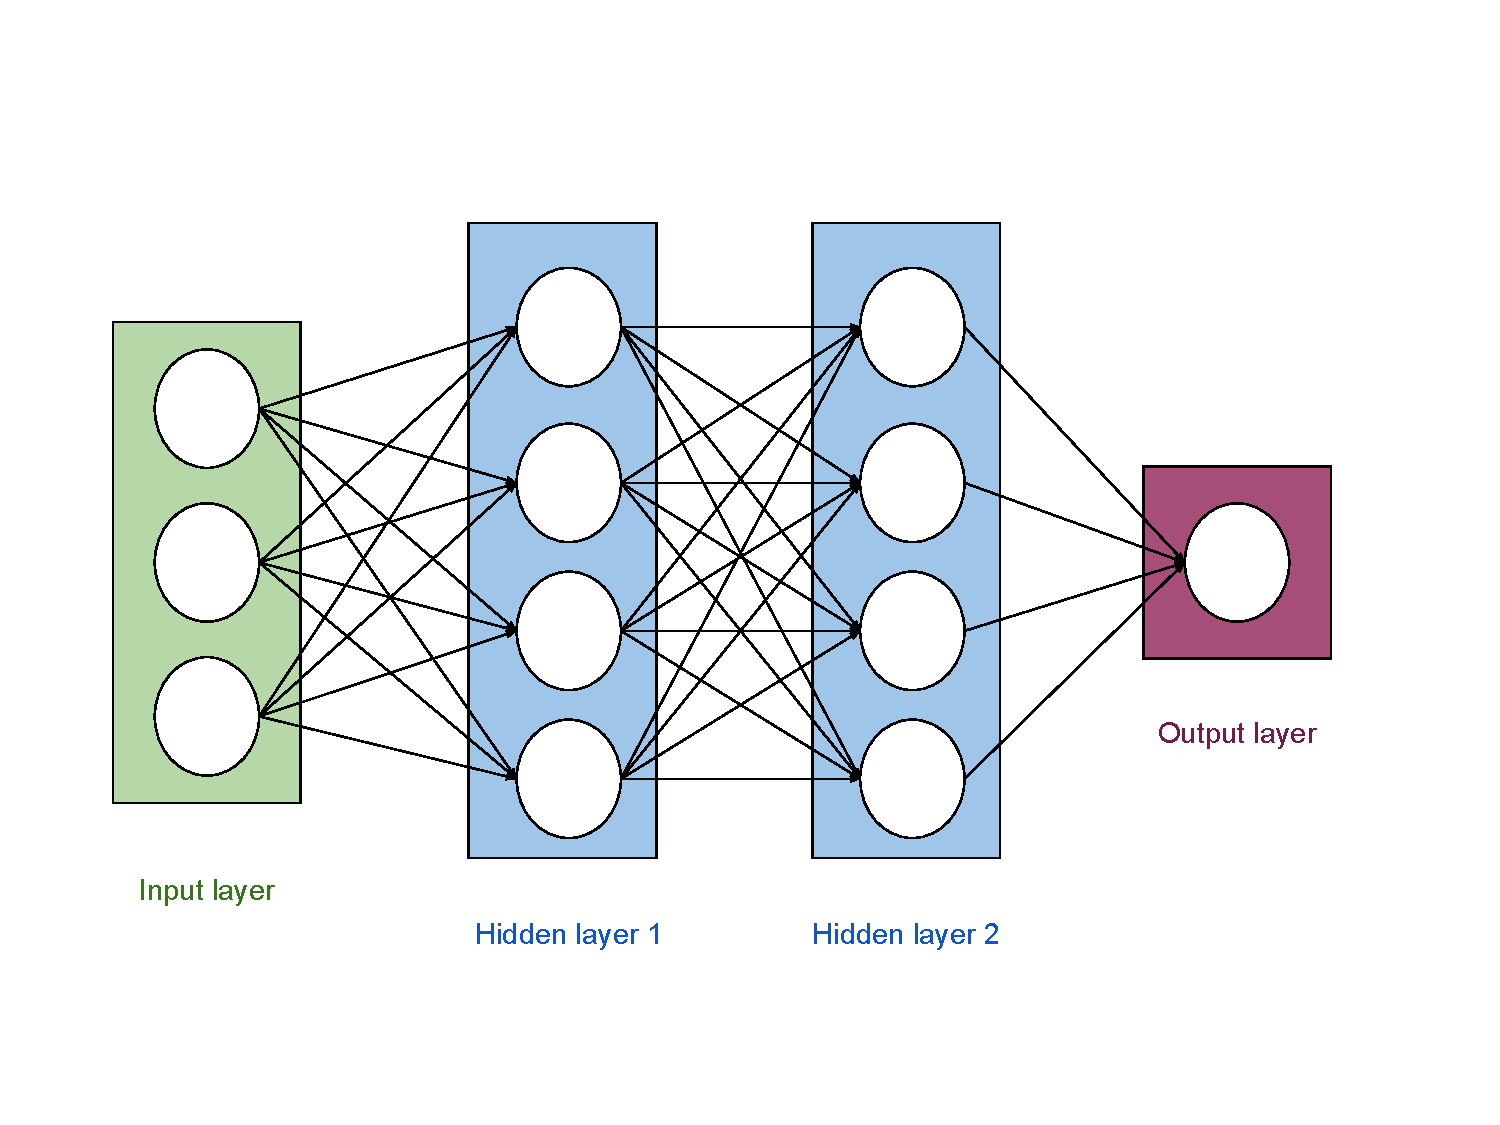
\includegraphics[height=.58\textheight]{Chapter2/Figs/MLP.pdf}
\label{fig:Two Layered Neural_Network}
\caption{Neural Network with two hidden layers}
\end{center}
\end{figure}


\subsection{Convolutional Neural Network}

Hubel and Wiesel in their hierarchy model mentioned a neural network to have a hierarchy structure in the visual cortex. LGB (lateral geniculate body) forms the simple cells that form the complex cells which form the lower order hypercomplex cells that finally form the higher order hypercomplex cells.
Also, the network between the lower order hypercomplex cells and the higher order hypercomplex cells are structurally similar to the network between simple cells and the complex cells. In this hierarchy, a cell in a higher stage generally has a tendency to respond selectively to a more complicated feature of the stimulus pattern, and the cell at the lower stage responds to simpler features. Also, higher stage cells possess a larger receptive field and are more insensitive to the shift in the position of the stimulus pattern.

Similar to a hierarchy model, a neural network starting layers learns simpler features like edges and corners and subsequent layers learn complex features like colours, textures and so on. Also, higher neural units possess a larger receptive field which builds over the initial layers. However, unlike in multilayer perceptron where all neurons from one layer are connected with all the neurons in the next layer, weight sharing is the main idea behind a convolutional neural network. 
Example: instead of each neuron having a different weight for each pixel of the input image (28*28 weights), the neurons only have a small set of weights (5*5) that is applied to a whole bunch of small subsets of the image of the same size. Layers past the first layer work in a similar way by taking in the ‘local’ features found in the previously hidden layer rather than pixel images, and successively see larger portions of the image since they are combining information about increasingly larger subsets of the image. Finally, the final layer makes the correct prediction for the output class.

The reason for why this is helpful is intuitive if not mathematically clear: without such constraints, the network would have to learn the same simple things (such as detecting edges, corners, etc) a whole bunch of times for each portion of the image. But with the constraint there, only one neuron would need to learn each simple feature - and with far fewer weights overall, it could do so much faster! Moreover, since the pixel-exact locations of such features do not matter the neuron could basically skip neighbouring subsets of the image - subsampling, now known as a type of pooling - when applying the weights, further reducing the training time. The addition of these two types of layers - convolutional and pooling layers - are the primary distinctions of Convolutional Neural Nets (CNNs/ConvNets) from plain old neural nets.


\section{Probabilistic Machine Learning}
\subsection{Variational Inference}

We define a function $y = f(\mathbf{x})$ that estimates the given inputs $\{ x_1, \hdots, x_N \}$ and their corresponding outputs $\{y_1, \hdots, y_N\}$ and produces an predictive output. Using Bayesian inference, a prior distribution is used over the space of functions $p(f)$. This distribution represents our prior belief as to which functions are likely to have generated our data. 

A likelihood is defined as $p(Y | f, X)$ to capture the process in which given a function observation is generated. We use the Bayes rule to find the posterior distribution given our dataset: $p(f | X, Y)$.

The new output can be predicted for a new input point $x^*$ by integrating over all possible functions $f$,
\begin{align} \label{eq:post}
%p(\f | \X, \Y) \propto p(\Y | \X, \f) p(\f).
p(y^* | x^*, X, Y) = \int p(y^* | f^*) p(f^* | x^*, X, Y) df^*
\end{align}

The equation \eqref{eq:post} is intractable due to the integration sign. We can approximate it by taking a finite set of random variables $w$ and conditioning the model on it. However, it is based on a modelling assumption that the model depends on these variables alone, and making them into sufficient statistics in our approximate model.

The predictive distribution for a new input point $x^*$ is then given by 
$$
p(y^* | x^*, X, Y) = \int p(y^* | f^*) p(f^* | x^*, w) p(w | X, Y) df^* d w.
$$

However, the distribution $p(w | X, Y)$ still remains intractable and we need to approximate it with a variational distribution $q(w)$, that can be computed. The approximate distribution needs to be as close as possible to the posterior distribution obtained from the original model. We thus minimise the Kullback--Leibler (KL) divergence, intuitively a measure of similarity between two distributions: $KL(q(w) ~||~ p(w | X, Y))$,
resulting in the approximate predictive distribution 
\begin{align} \label{eq:predictive}
q(y^* | x^*) = \int p(y^* | f^*) p(f^* | x^*, w) q(w)  df^* dw.
\end{align}

Minimising the Kullback--Leibler divergence is equivalent to maximising the \textit{log evidence lower bound},
\begin{align}
KL_{\text{VI}} := \int q(w) p(F | X, w) \log p(Y | F) dF dw - \KL(q(w) || p(w)) \label{eq:L:VI}
\end{align}
with respect to the variational parameters defining $q(w)$. This is known as \textit{variational inference}, a standard technique in Bayesian modelling.

Maximizing the KL divergence between the posterior and the prior over $w$ will result in a variational distribution that learns a good representation from the data (obtained from log likelihood) and is closer to the prior distribution. In other words, it can prevent overfitting. 


\subsection{Local  Reparametrisation  Trick}
The ability to rewrite statistical problems in an equivalent but different form, to reparameterise them, is one of the most general-purpose tools used in mathematical statistics. The type of \textit{reparameterization} when the global uncertainty in the weights is translated into a form of local uncertainty which is independent across examples is known as the \emph{local reparameterization trick}. 
An alternative estimator is deployed for which $\Cov{}{L_{i},L_{j}} = 0$, so that the variance of the stochastic gradients scales as $1/M$.
The new estimator is made computationally efficient by sampling the intermediate variables and not sampling $\beps$ directly, but only  $f(\beps)$ through which $\beps$ influences $L_\D^\text{SGVB}(\bphi)$. Hence, the source of global noise can be translated to local noise ($\beps \rightarrow f(\beps)$), a local reparameterization can be applied so as to obtain a statistically efficient gradient estimator.

The technique can be explained through a simple example: We consider an input($X$) of random uniform function ranging from -1 to +1 and an output($Y$) as a random normal distribution around mean $X$ and standard deviation $\delta$. The Mean Squared Loss would be defined as 
$(Y-X)^2$. The problem here is during the backpropagation from the random normal distribution function. As we are trying to propagate through a stochastic node we reparameterize by adding $X$ to the random normal function output and multiplying by $\delta$.
The movement of parameters out of the normal distribution does not change the behaviour of the model. 


\section{Uncertainties in Bayesian Learning}


Uncertainties in a network is a measure of how certain the model is with its prediction. In Bayesian modelling, there are two main types of uncertainty one can model \citep{Kiureghian}: \textit{Aleatoric} uncertainty and \textit{Epistemic} uncertainty. 

\textit{Aleatoric} uncertainty measures the noise inherent in the observations. This type of uncertainty is present in the data collection method like the sensor noise or motion noise which is uniform along the dataset. This cannot be reduced if more data is collected. \textit{Epistemic} uncertainty, on the other hand, represents the uncertainty caused by the model. This uncertainty can be reduced given more data and is often referred to as \textit{model uncertainty}.  Aleatoric uncertainty can further be categorized into \textit{homoscedastic} uncertainty, uncertainty which stays constant for different inputs, and \textit{heteroscedastic} uncertainty. Heteroscedastic uncertainty depends on the inputs to the model, with some inputs potentially having more noisy outputs than others. Heteroscedastic uncertainty is in particular important so that model prevents from outputting very confident decisions.

Current work measures uncertainties by placing a probability distributions over either the model parameters or model outputs. Epistemic uncertainty is modelled by placing a prior distribution over a model's weights and then trying to capture how much these weights vary given some data. Aleatoric uncertainty, on the other hand, is modelled by placing a distribution over the output of the model.

\subsubsection{Sources of Uncertainities}

The following can be the source of uncertainty as mentioned by Kiureghian \cite{Kiureghian}:

\begin{enumerate}
    \item Uncertainty inherent in the basic random variables $X$, such as the uncertainty inherent in material property constants and load values, which can be directly measured.
    \item Uncertain model error resulting from the selection of the form of the probabilistic sub-model $f_{X}(x,H_{f})$ used to describe the distribution of basic variables.
    \item  Uncertain modeling errors resulting from selection of the physical sub-models $g_{i}(x,H_{g}), i = 1,2,...,m,$ used to describe the derived variables.
    \item  Statistical uncertainty in the estimation of the parameters $H_f$ of the probabilistic sub-model.
    \item  Statistical uncertainty in the estimation of the parameters $H_g$ of the physical sub-models.
    \item  Uncertain errors involved in measuring of observations, based on which the parameters $H_f$ and $H_g$  are estimated. These include errors involved in indirect measurement, e.g., the measurement of a quantity through a proxy, as in non-destructive testing of material strength.
    \item Uncertainty modelled by the random variables $Y$ corresponding to the derived variables $y$, which may include, in addition to all the above uncertainties, uncertain errors resulting from computational errors, numerical approximations or truncations. For example, the computation of load effects in a nonlinear structure by a finite element procedure employs iterative calculations, which invariably involve convergence tolerances and truncation errors.
\end{enumerate} 

\section{Backpropagation}

Backpropagation in a Neural Networks was proposed by Rumelhart \cite{Rumelhart} in 1986 and it is the most commonly used method for training neural networks. Backpropagation is a technique to compute the gradient of the loss in terms of the network weights. It operates in two phases: firstly, the input features through the network propagates in the forward direction to compute the function output and thereby the loss associated with the parameters. Secondly, the derivatives of the training loss with respect to the weights
are propagated back from the output layer towards the input layers.
These computed derivatives are further used to update the weights of the network. This is a continuous process and updating of the weight occurs continuously over every iteration. 

Despite the popularity of backpropagation, there are many hyperparameters in backpropagation based stochastic optimization that requires specific tuning, e.g., learning rate, momentum, weight decay, etc. The time required for finding the optimal values is proportional to the data size. For a network trained with backpropagation, only point estimates of the weights are achieved in the network. As a result, these networks make overconfident predictions and do not account for uncertainty in the parameters. Lack of uncertainty measure makes the network prone to overfitting and a need for regularization.

A Bayesian approach to Neural Networks provides the shortcomings with the backpropagation approach \cite{mackay1996hyperparameters} as Bayesian methods naturally account for uncertainty in parameter estimates and can propagate this uncertainty into predictions.
Also, averaging over parameter values instead of just choosing single point estimates makes the model robust to overfitting. 

Sevreal approaches has been proposed in the past for learning in Bayesian Networks: Laplace approximation \cite{Mackay1991APB}, MC Dropout \cite{gal2015bayesian},and Variational Inference \cite{hinton1993keeping} \cite{graves2011practical} \cite{blundell2015weight}. We used Bayes by Backprop \cite{blundell2015weight} for our work and is explained next.

\subsection{Bayes by Backprop}
\textit{Bayes by Backprop} \cite{graves2011practical, blundell2015weight} is a variational inference method to learn the posterior distribution on the weights $w \sim q_{\theta}(w|\mathcal{D})$ of a neural network from which weights $w$ can be sampled in backpropagation. 
It regularises the weights by minimising a compression cost, known as the variational free energy or the expected lower bound on the marginal likelihood.

Since the true posterior is typically intractable, an approximate distribution $q_{\theta}(w|\mathcal{D})$ is defined that is aimed to be as similar as possible to the true posterior $p(w|\mathcal{D})$, measured by the Kullback-Leibler (KL) divergence \cite{kullback1951information}. Hence, we define the optimal parameters $\theta^{opt}$ as
\begin{equation}
    \begin{aligned} \label{KL}
        \theta^{opt}&=\underset{\theta}{\text{arg min}}\ \text{KL} \ [q_{\theta}(w|\mathcal{D})\|p(w|\mathcal{D})] \\
        &=\underset{\theta}{\text{arg min}}\ \text{KL} \ [q_{\theta}(w|\mathcal{D})\|p(w)] \\ & -\mathbb{E}_{q(w|\theta)}[\log p(\mathcal{D}|w)]+\log p(\mathcal{D})
    \end{aligned}
\end{equation}

where
\begin{equation}
    \text{KL} \ [q_{\theta}(w|\mathcal{D})\|p(w)]= \int q_{\theta}(w|\mathcal{D})\log\frac{q_{\theta}(w|\mathcal{D})}{p(w)}dw .
\end{equation}
This derivation forms an optimisation problem with a resulting cost function widely known as \textit{variational free energy} \cite{neal1998view,yedidia2005constructing,friston2007variational} which is built upon two terms: the former, $\text{KL} \ [q_{\theta}(w|\mathcal{D})\|p(w)]$, is dependent on the definition of the prior $p(w)$, thus called complexity cost, whereas the latter, $\mathbb{E}_{q(w|\theta)}[\log p(\mathcal{D}|w)]$, is dependent on the data $p(\mathcal{D}|w)$, thus called likelihood cost. 
The term $\log p(\mathcal{D})$ can be omitted in the optimisation because it is constant.
\newline Since the KL-divergence is also intractable to compute exactly, we follow a stochastic variational method \cite{graves2011practical,blundell2015weight}.
We sample the weights $w$ from the variational distribution $q_{\theta}(w|\mathcal{D})$ since it is much more probable to draw samples which are appropriate for numerical methods from the variational posterior $q_{\theta}(w|\mathcal{D})$ than from the true posterior $p(w|\mathcal{D})$. Consequently, we arrive at the tractable cost function \eqref{cost} which is aimed to be optimized, i.e. minimised w.r.t. $\theta$, during training:
\begin{equation} \label{cost}
    \mathcal{F}(\mathcal{D}, \theta)\approx \sum_{i=1}^n \log q_{\theta}(w^{(i)}|\mathcal{D})-\log p(w^{(i)})-\log p(\mathcal{D}|w^{(i)})
\end{equation}
%
where $n$ is the number of draws.
\newline We sample $w^{(i)}$ from $q_{\theta}(w|\mathcal{D})$. The uncertainty afforded by \textit{Bayes by Backprop} trained neural networks has been used successfully for training feedforward neural networks in both supervised and reinforcement learning environments \cite{blundell2015weight,lipton2016efficient,houthooft2016curiosity}, for training recurrent neural networks \cite{fortunato2017bayesian}, but has not been applied to convolutional neural networks to-date.

\section{Model Weights Pruning}

Model pruning reduces the sparsity in a deep neural network's
various connection matrices, thereby reducing the number of valued parameters in the model. The whole idea of model pruning is to reduce the number of parameters without much loss in the accuracy of the model. This reduces the use of a large parameterized model with regularization and promotes the use of dense connected smaller models. Some recent work suggests \cite{DBLP:journals/corr/HanMD15} \cite{DBLP:journals/corr/NarangDSE17} that the network can achieve a sizable reduction in model size, yet achieving comparable accuracy. 
Model pruning possesses several advantages in terms of reduction in computational cost, inference time and in energy-efficiency. The resulting pruned model typically has sparse connection matrices, so
efficient inference using these sparse models requires purpose-built hardware capable of loading sparse matrices and/or performing sparse matrix-vector operations. Thus the overall memory usage is reduced with the new pruned model. 


There are several ways of achieving the pruned model, the most popular one is to map the low contributing weights to zero and reducing the number of overall non-zero valued weights. This can be achieved by training a large sparse model and pruning it further which makes it comparable to training a small dense model. Pruning away the less salient features to zero has been used in this thesis and is explained in details in Chapter 4. 


